\section{Experimental Setup}
The following equipment, as described in this section, can be seen on
\cref{fig_setup1}, \cref{fig_setup2} and \cref{fig_setup3}.

We will be accelerating particles by the Van-de-Graaf accelerator up to $
\SI{400}{\kilo\electronvolt}$. The variety of incomming particles are limited
by the source, which is a flask of gas connected to the accelerator tank. We
will not change this flask, for which our experiment is limited to protons, and
the hydrogenic ions: $H^{+}$ and $H^{++}$. By changing the magnetic field, one
can choose which of these particles will interact with the target.

When calibrating, 

\subsection{Calibration}



\begin{figure}[h]
\centering
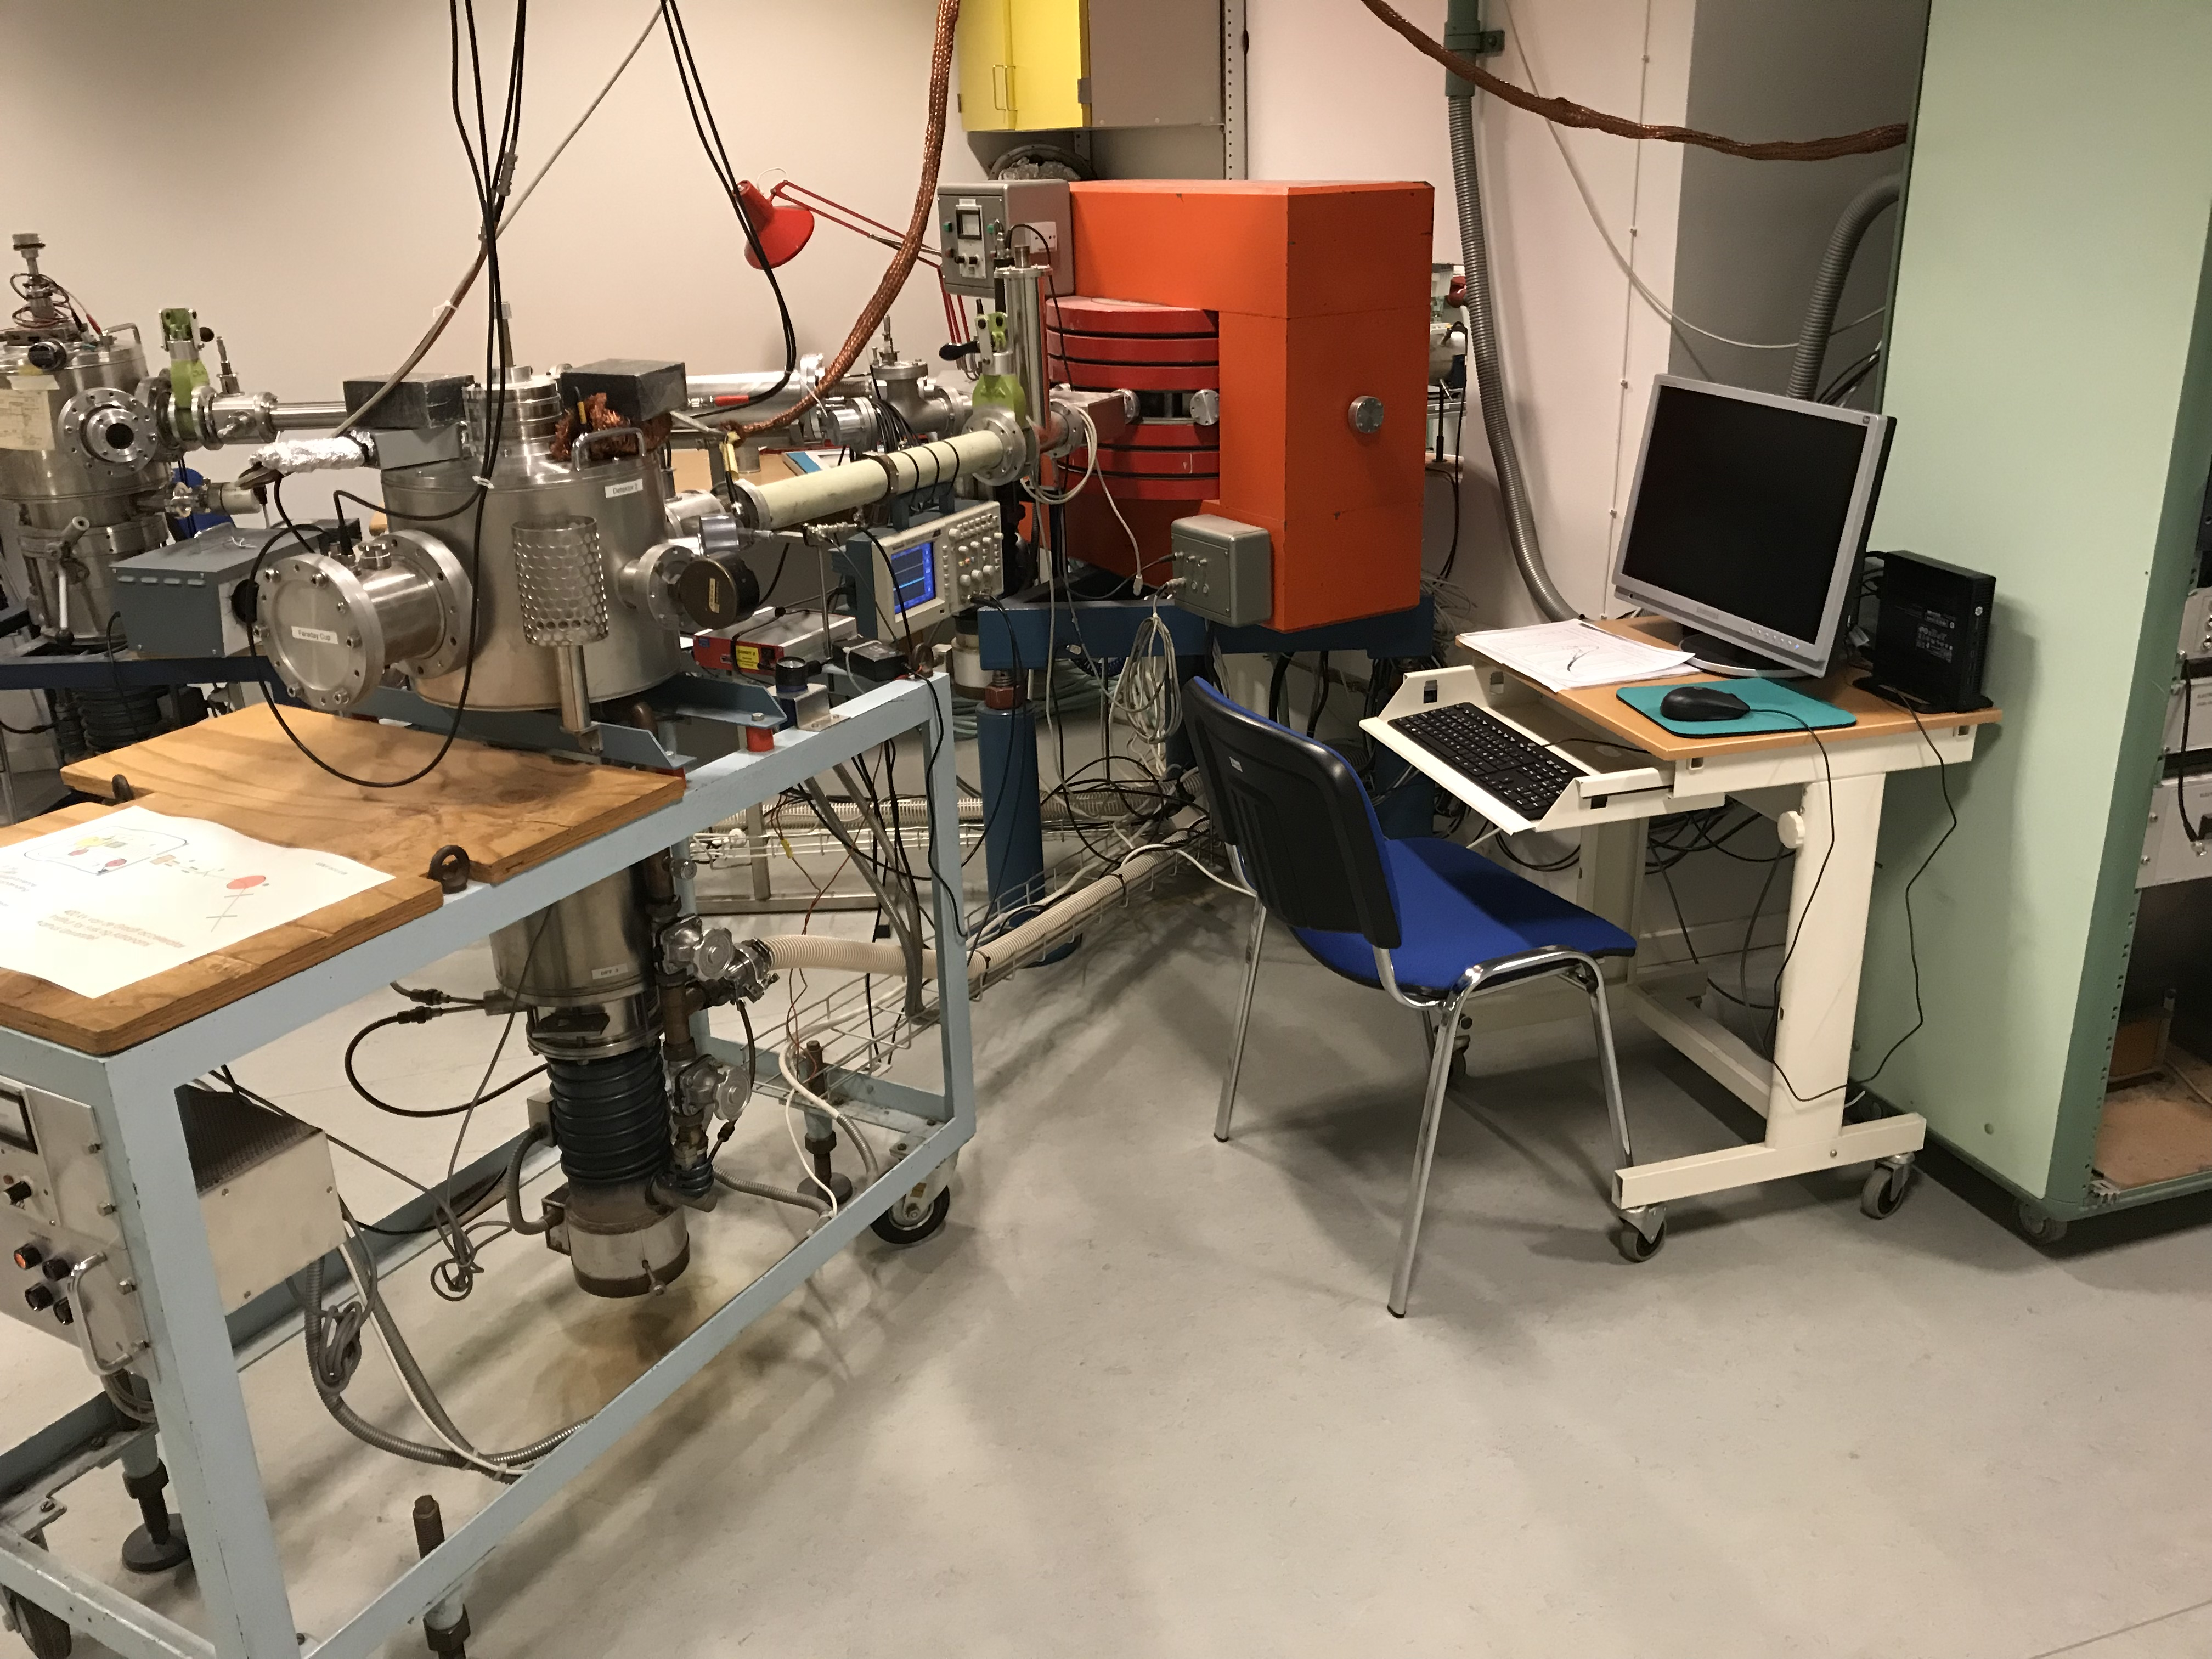
\includegraphics[width=0.5\textwidth]{setup1}
\caption{Experimental setup 1: The detector and a computer for the data
analysis.}
\label{fig_setup1}
\end{figure}

\begin{figure}[h]
\centering
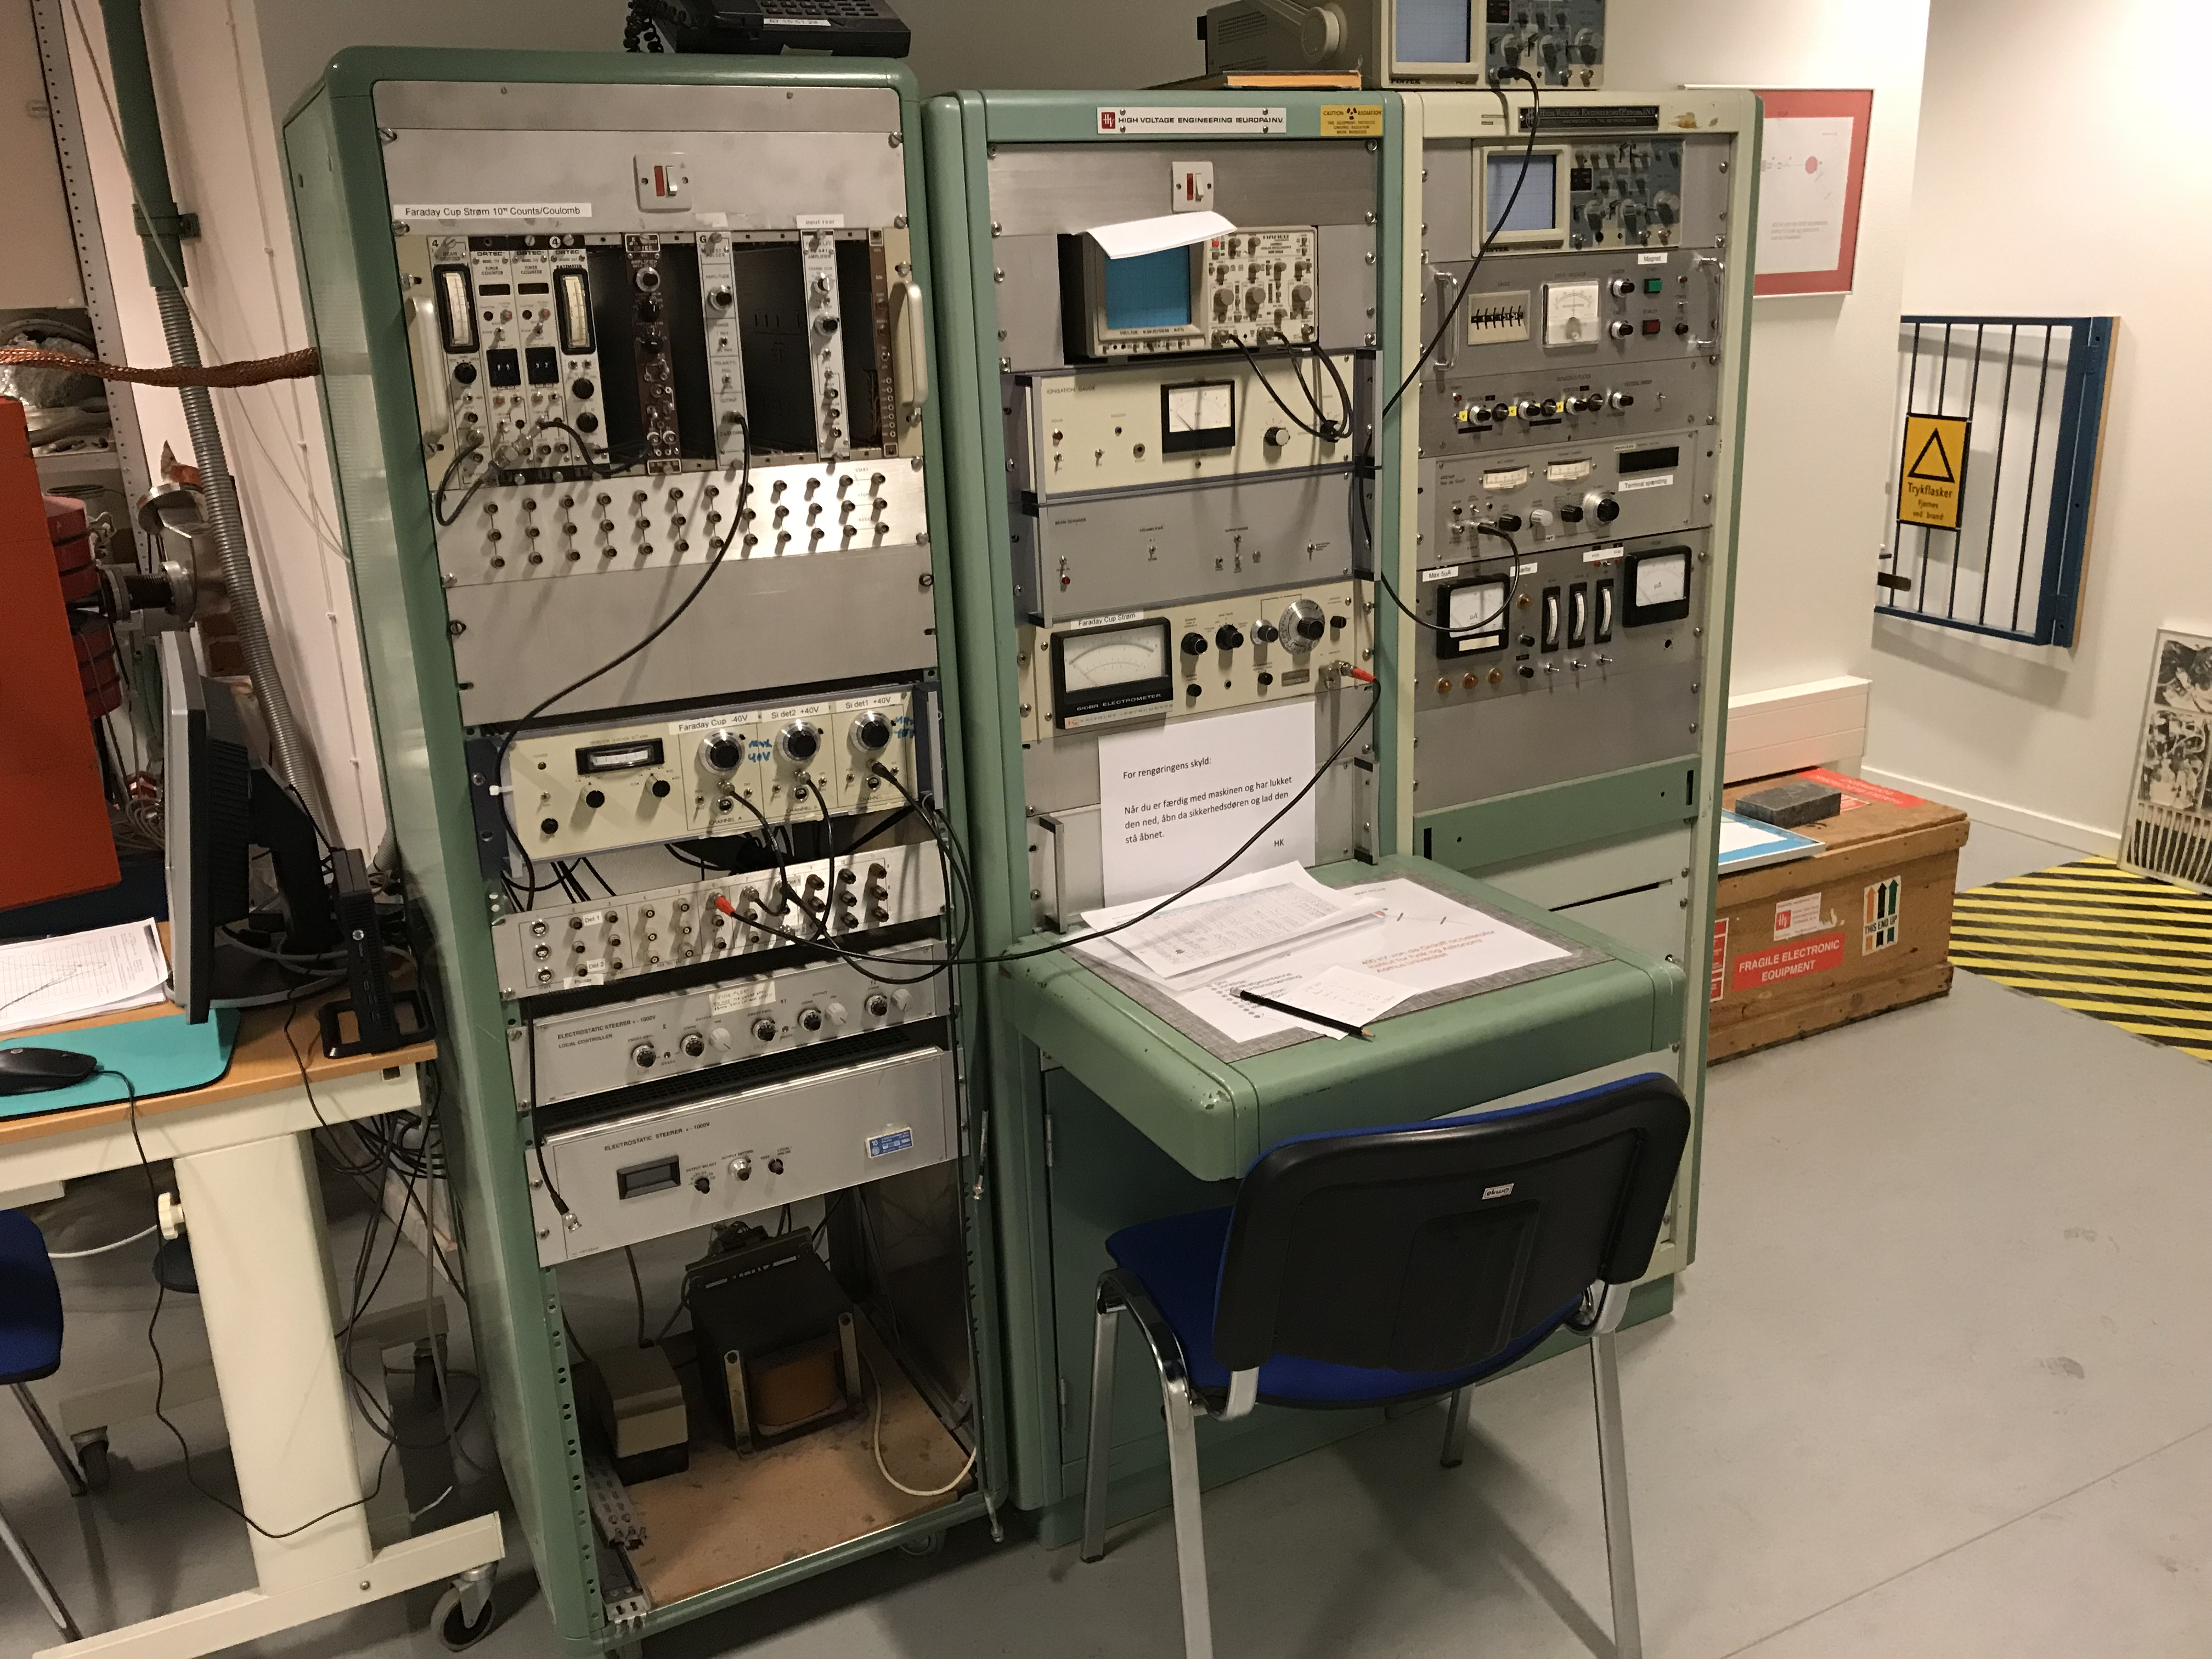
\includegraphics[width=0.5\textwidth]{setup2}
\caption{Experimental setup 2: All components with variables.}
\label{fig_setup2}
\end{figure}

\begin{figure}[h]
\centering
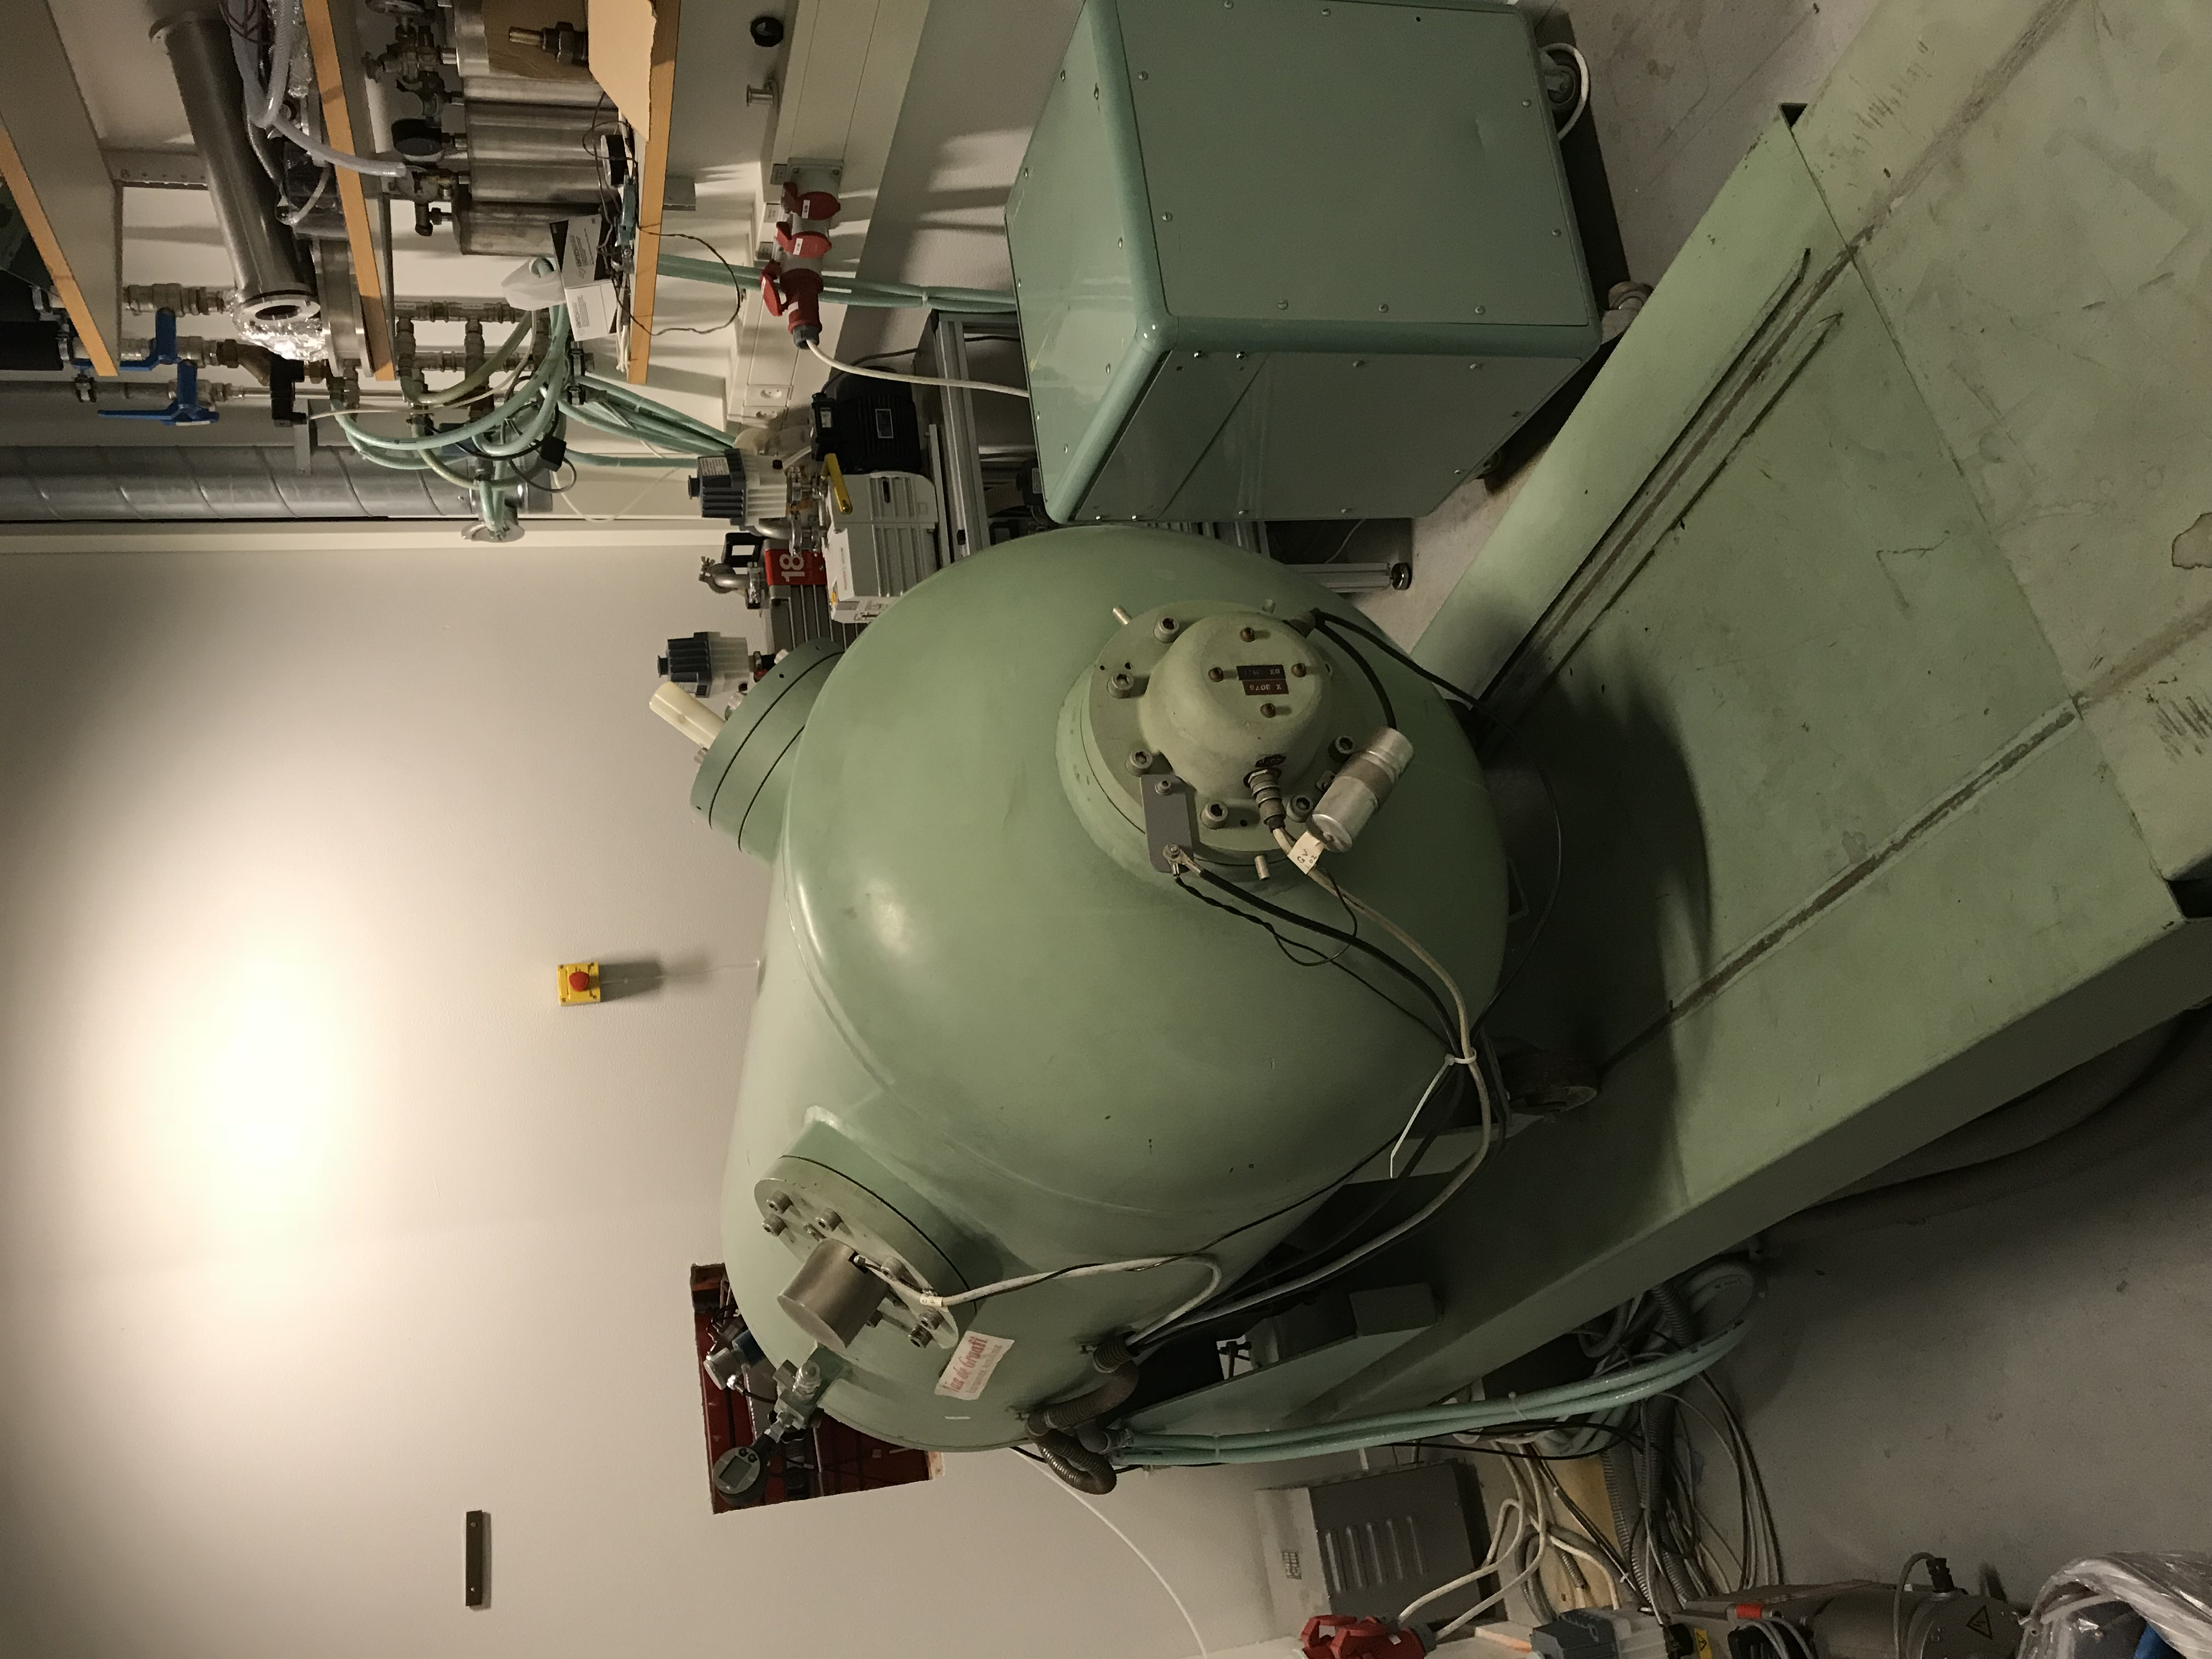
\includegraphics[width=0.5\textwidth]{setup3}
\caption{Experimental setup 3: The single Van-de-Graaf accelerator.}
\label{fig_setup3}
\end{figure}

